\section{Ergebnisse aus der Simulatorrecherche}\label{chap:results_sim}

\sh{Allgemeine Informationen}
Abbildung~\ref{fig:1-anzahl-jahr} verdeutlicht, dass der Großteil der untersuchten Simulatoren zu Beginn der 2000er-Jahre veröffentlicht wurde. Zwischen 2000 und 2020 lassen sich insgesamt 37 Veröffentlichungen identifizieren, was einem Anteil von 74~\% entspricht. Darüber hinaus konnte bei sieben Simulatoren kein Veröffentlichungsdatum ermittelt werden.

Hinsichtlich des Wartungsstands der bereits veröffentlichten Simulatoren zeigt Abbildung~\ref{fig:2-veroeffentlichungen}, dass dieser im Zeitverlauf zunimmt. Etwa 71~\% der Simulatoren wurden in den vergangenen fünf Jahren aktualisiert und können somit als regelmäßig gepflegt eingestuft werden.

\begin{figure}[!htbp]
    \centering
    % --- linke Seite: Grafik ---
    \begin{subfigure}[b]{0.48\textwidth}
        \centering
        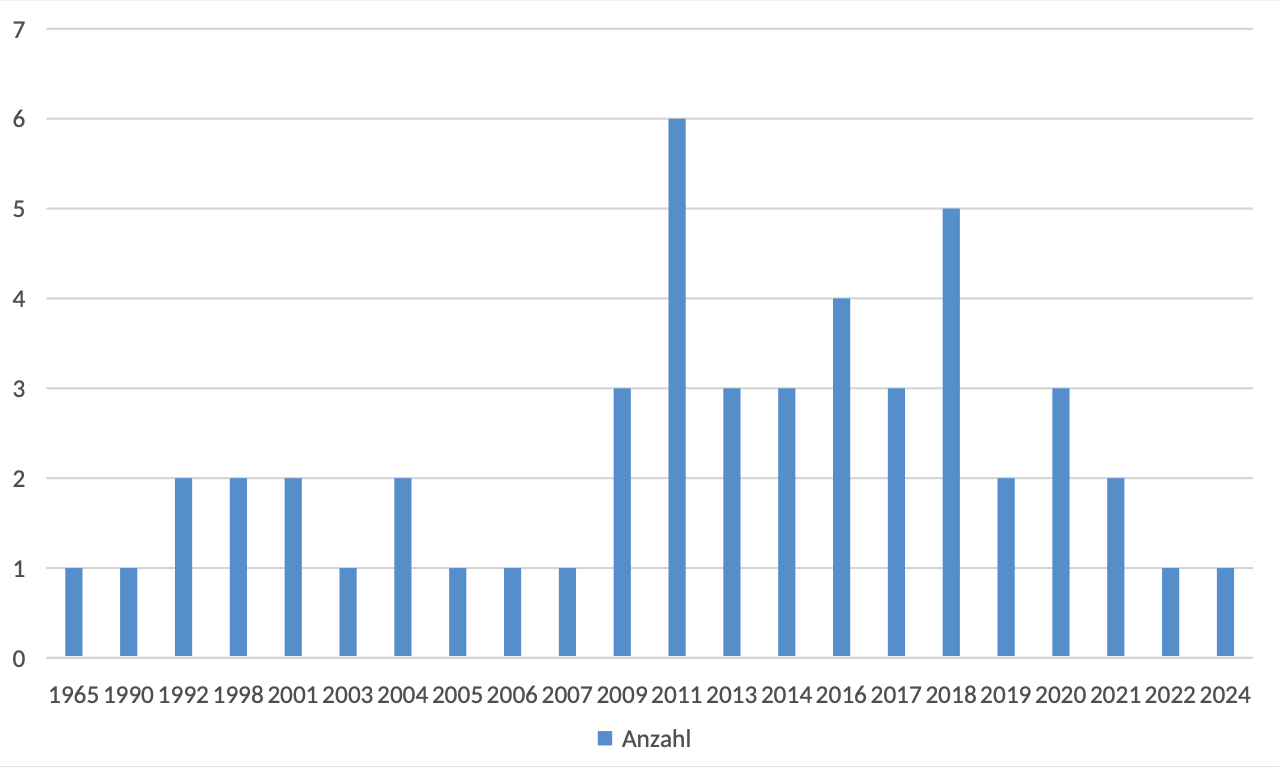
\includegraphics[width=0.90\textwidth]{graphics_sim/1-anzahl-jahr.png}
        \caption{Jährliche Übersicht der Veröffentlichungen}
        \label{fig:1-anzahl-jahr}
    \end{subfigure}
    \hfill
    % 
    % --- rechte Seite: Grafik ---
    \begin{subfigure}[b]{0.48\textwidth}
        \centering
        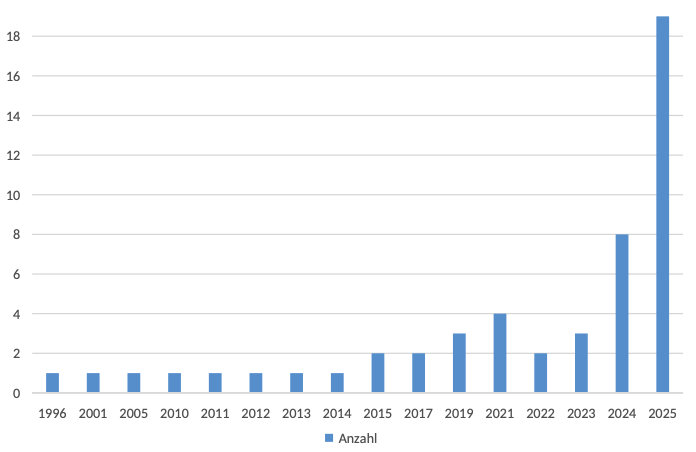
\includegraphics[width=0.90\textwidth]{graphics_sim/2-veroeffentlichung.png}
        \caption{Jährliche Übersicht des Wartungsstands}
        \label{fig:2-veroeffentlichungen}
    \end{subfigure}
    %
    \caption{Übersicht der Veröffentlichungen und des Wartungsstands pro Jahr (Simulator)}
    \label{fig:veroeffentlichung_wartungsstand}
\end{figure}

\sh{Chronologische Entwicklung}
Die thematische Verteilung der Simulatoren ist Abbildung~\ref{fig:7-thema} zu entnehmen. Etwa 40~\% der Simulatoren befassen sich mit dem Themenbereich \enquote{Prozessoren und Architekturen}, gefolgt von 18~\% hardwarebezogenen und 14~\% grundlagenvermittelnden Simulatoren. Die übrigen Anwendungen verteilen sich auf die Themenbereiche \enquote{Speicher und Performance}, \enquote{Programmierung}, \enquote{Systeme und Anwendungen}, \enquote{GPU} sowie \enquote{Monitoring}.

Die Zuordnung der Veröffentlichungsjahre zu den Zeiträumen \enquote{vor 2000}, \enquote{2000 -- 2010}, \enquote{2010 -- 2020} und \enquote{nach 2020} ist in Abbildung~\ref{fig:8-thema-jahr} dargestellt. Hier wird deutlich, dass die Mehrheit der Simulatoren zum Themenbereich \enquote{Prozessoren und Architekturen} im Zeitraum 2010 bis 2020 veröffentlicht wurde.

Wie bereits in der Literaturrecherche sind auch in der Simulatorrecherche die Themenbereiche \enquote{Prozessoren und Architekturen} sowie \enquote{Hardware und Logik} am stärksten vertreten. Unter den 49~\% der untersuchten Simulatoren treten insbesondere die Subthemen \enquote{\acs{RISC}} und \enquote{Digitale Logik} am häufigsten auf. Damit lassen sich vergleichbare Entwicklungen in beiden Analysen feststellen.

Die verbleibenden Themenbereiche liefern in Bezug auf die zeitliche Entwicklung anhand des Veröffentlichungsjahres keine weiterführenden Erkenntnisse. Auch aus dem Wartungsstand der untersuchten Simulatoren lassen sich keine eindeutigen Trends ableiten. Wie Abbildung~\ref{fig:2-veroeffentlichungen} zeigt, befinden sich die meisten Simulatoren im Wesentlichen auf einem aktuellen Entwicklungsstand. Das gewichtete arithmetische Mittel des Wartungsstands pro Themenbereich liegt nicht vor dem Jahr 2018.


\begin{figure}[!htbp]
    \centering
    % --- linke Seite: Grafik ---
    \begin{subfigure}[b]{0.48\textwidth}
        \centering
        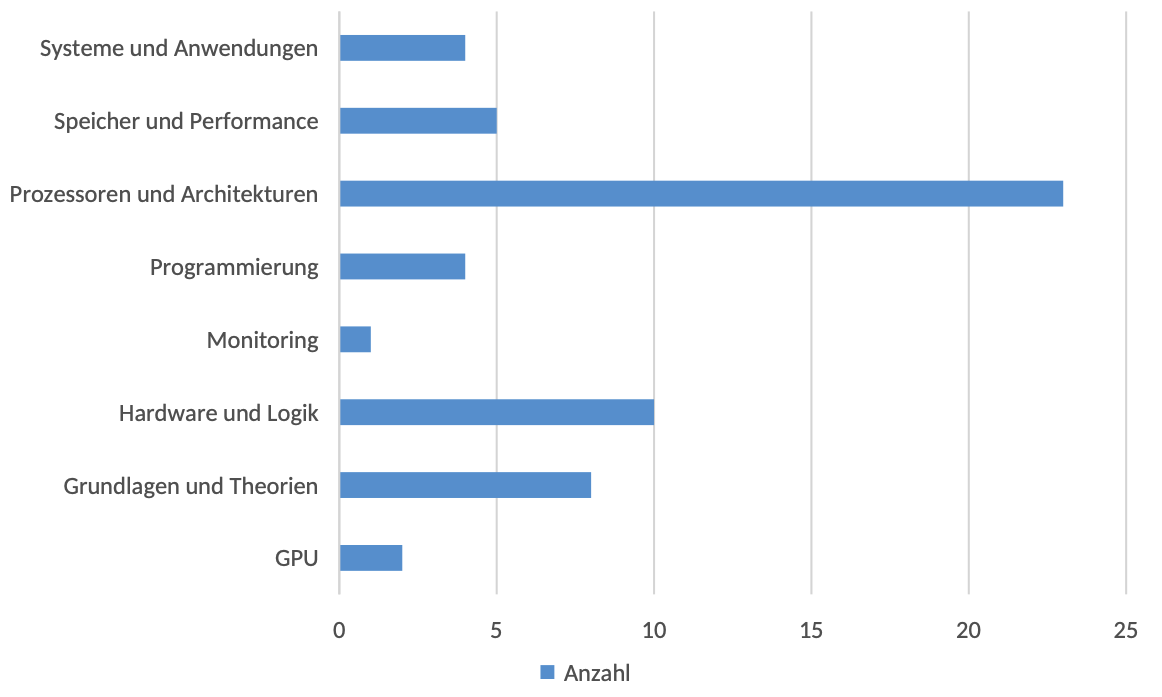
\includegraphics[width=0.90\textwidth]{graphics_sim/7-thema.png}
        \caption{Übersicht der Themenverteilung}
        \label{fig:7-thema}
    \end{subfigure}
    \hfill
    % 
    % --- rechte Seite: Grafik ---
    \begin{subfigure}[b]{0.48\textwidth}
        \centering
        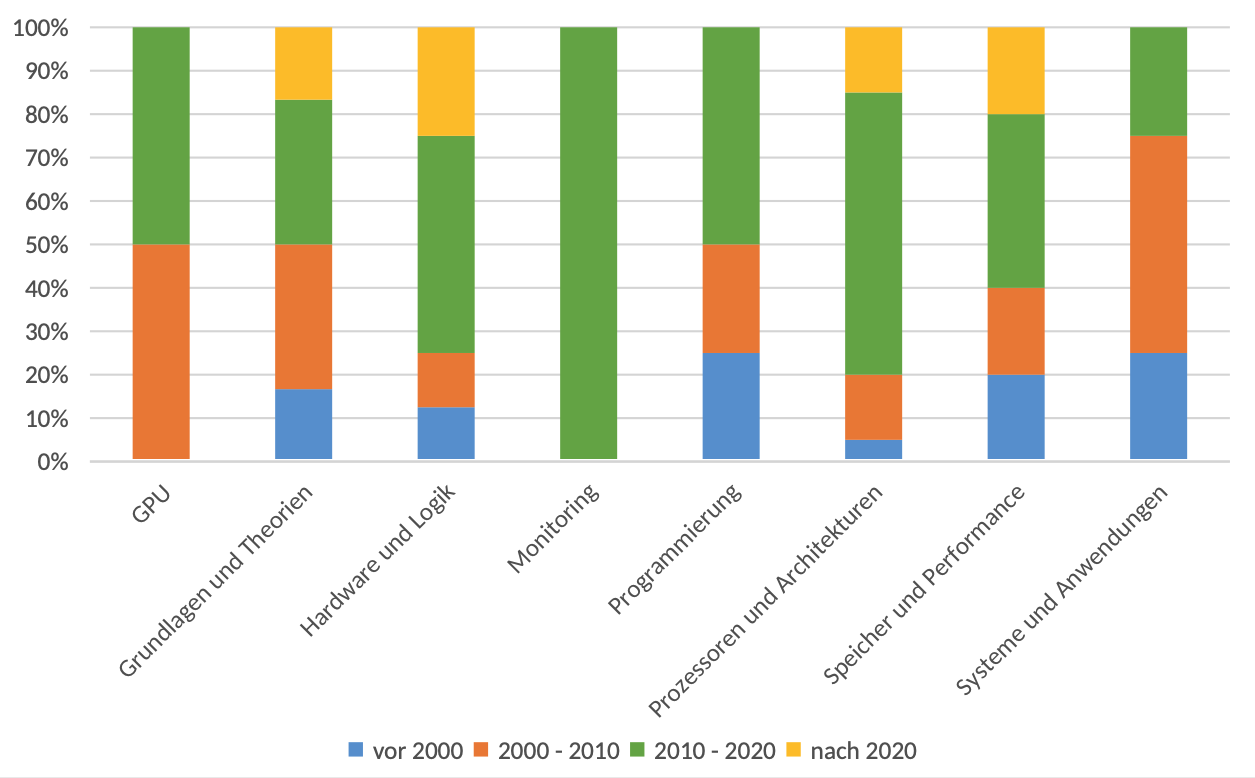
\includegraphics[width=0.90\textwidth]{graphics_sim/8-thema-jahr.png}
        \caption{Jährliche Übersicht der Themenverteilung}
        \label{fig:8-thema-jahr}
    \end{subfigure}
    %
    \caption{Analysen zur Themenverteilung (Simulator)}
    \label{fig:themen-gesamt}
\end{figure}

\sh{Gamification}
Hinsichtlich des Kriteriums Gamification zeigt die Analyse, dass die in Tabelle~\ref{tab:simulatoren} aufgeführten Simulatoren keine spielerischen Elemente enthalten. Eine Bewertung dieses Kriteriums ist daher auf Grundlage der vorliegenden Daten nicht möglich.

\sh{Abstraktionslevel}
Im Rahmen der Simulatorrecherche wird auch das Abstraktionsniveau erfasst (vgl. Abbildung~\ref{fig:5-abstraktion}). Der überwiegende Teil (ca. 72~\%) der Simulatoren ist dabei als \enquote{didaktisch reduziert} zu klassifizieren. Diese Simulatoren verteilen sich gemäß Abbildung~\ref{fig:6-abstraktion-thema} im Wesentlichen auf die Themenbereiche \enquote{Prozessoren und Architekturen} sowie \enquote{Hardware und Logik}.

\begin{figure}[!htbp]
    \centering
    % --- linke Seite: Grafik ---
    \begin{subfigure}[b]{0.48\textwidth}
        \centering
        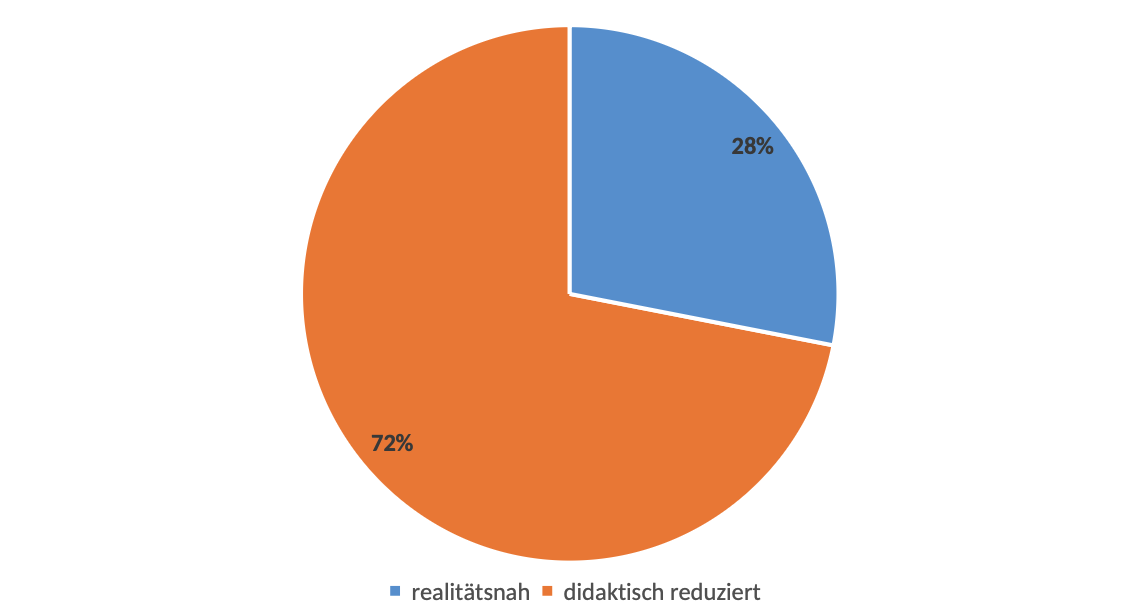
\includegraphics[width=0.90\textwidth]{graphics_sim/5-abstraktion.png}
        \caption{Übersicht der Abstraktionslevel}
        \label{fig:5-abstraktion}
    \end{subfigure}
    \hfill
    % 
    % --- rechte Seite: Grafik ---
    \begin{subfigure}[b]{0.48\textwidth}
        \centering
        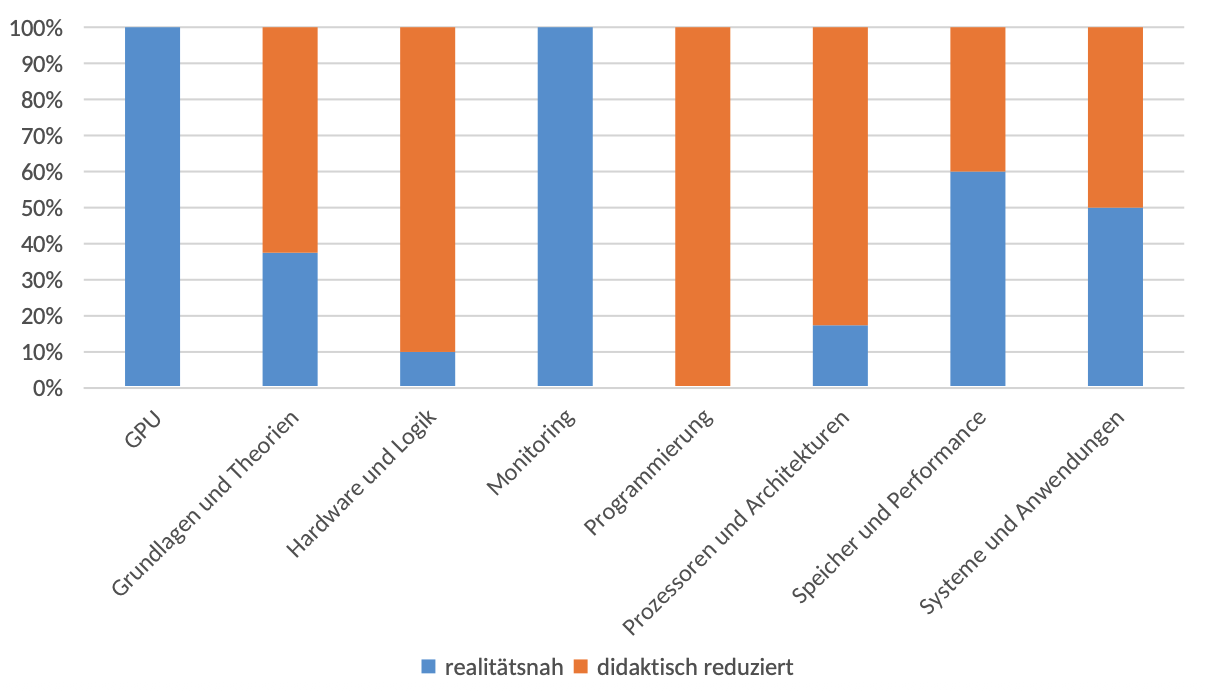
\includegraphics[width=0.90\textwidth]{graphics_sim/6-abstraktion-thema.png}
        \caption{Übersicht der Abstraktionslevel pro Thema}
        \label{fig:6-abstraktion-thema}
    \end{subfigure}
    %
    \caption{Analysen zum Abstraktionslevel (Simulator)}
    \label{fig:abstraktion-gesamt}
\end{figure}

Neben dem Abstraktionsniveau wird auch die Zielgruppe der jeweiligen Simulatoren (Kriterium \enquote{Institution}) betrachtet. Dabei erfolgt eine Unterscheidung zwischen den Kategorien \enquote{Schule}, \enquote{Hochschule} sowie \enquote{Forschung, Beruf}. Da eine Anwendung potenziell für mehrere Zielgruppen relevant sein kann und somit mehreren Kategorien zugeordnet wird, wird auf eine grafische Darstellung verzichtet. Tabelle~\ref{tab:institutionen} bietet stattdessen eine Übersicht über die Verteilung der Simulatoren auf die jeweiligen Institutionstypen.

\begin{table}[h]
	\centering
	\caption{Verteilung der Institutionen (Simulator)}
	\label{tab:institutionen}
	\begin{tabular}{l r}
		\toprule
		\textbf{Institution(en)} & \textbf{Anzahl} \\
		\midrule
		Schule                        & 7  \\
		Schule, Hochschule            & 2  \\
		Hochschule                    & 31 \\
		Hochschule, Forschung, Beruf  & 14 \\
		Forschung, Beruf              & 3  \\
        \hline
        \textbf{Summe}                & \textbf{57} \\
		\bottomrule
	\end{tabular}
\end{table}

Analog zur Literaturrecherche zeigt auch die Analyse der Simulatoren, dass der überwiegende Teil didaktisch reduziert ist. Eine Ausnahme bilden die Themenbereiche \enquote{GPU} und \enquote{Monitoring}, in denen ausschließlich realitätsnahe Simulatoren vorliegen.

Die Annahme, dass Simulatoren für die Hochschulbildung überwiegend didaktisch reduziert sein sollten, wird durch die Grundgesamtheit der veröffentlichten Systeme bestätigt: 72~\% der identifizierten Simulatoren sind didaktisch reduziert und richten sich an die Zielgruppen \enquote{Schule} und \enquote{Hochschule}.

Vor diesem Hintergrund ist das Kriterium \enquote{Vorwissen} von besonderem Interesse. Etwa 77~\% der Simulatoren setzen Grundkenntnisse in den jeweiligen Themengebieten voraus (vgl. Abbildung~\ref{fig:10-vorwissen}), rund 5~\% erfordern fortgeschrittene Kenntnisse, während lediglich 18~\% ohne Vorkenntnisse genutzt werden können. Die Verteilung nach Themengebieten in Abhängigkeit vom erforderlichen Vorwissen ist in Abbildung~\ref{fig:11-vorwissen-thema} dargestellt.

\begin{figure}[!htbp]
    \centering
    % --- linke Seite: Grafik ---
    \begin{subfigure}[b]{0.48\textwidth}
        \centering
        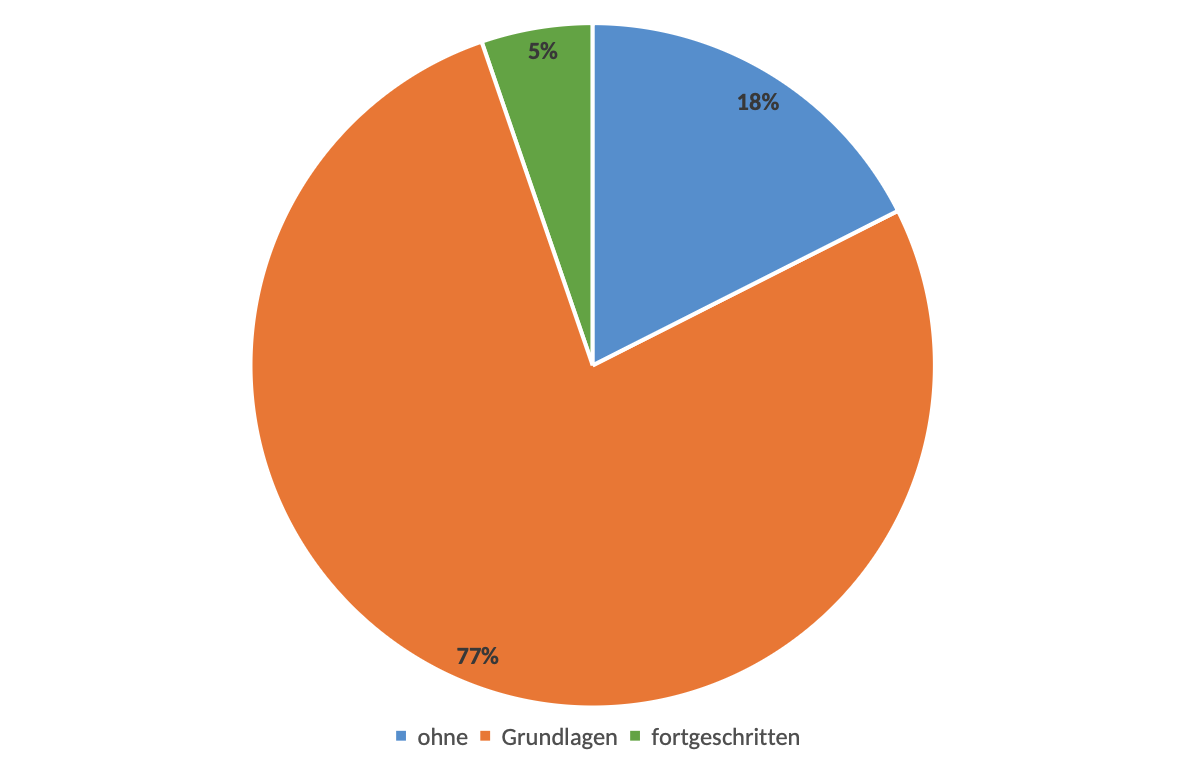
\includegraphics[width=0.90\textwidth]{graphics_sim/10-vorwissen.png}
        \caption{Verteilung Vorwissen}
        \label{fig:10-vorwissen}
    \end{subfigure}
    \hfill
    % 
    % --- rechte Seite: Grafik ---
    \begin{subfigure}[b]{0.48\textwidth}
        \centering
        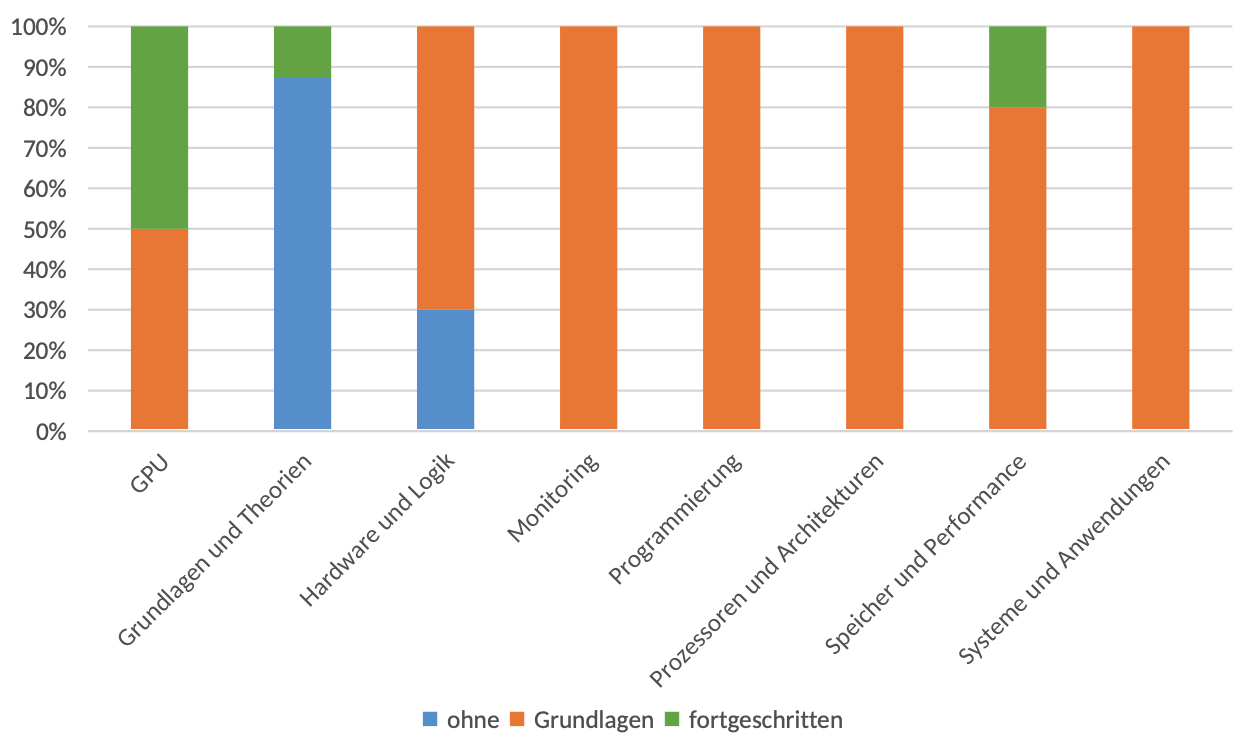
\includegraphics[width=0.90\textwidth]{graphics_sim/11-vorwissen-thema.png}
        \caption{Verteilung Vorwissen auf Themen}
        \label{fig:11-vorwissen-thema}
    \end{subfigure}
    %
    \caption{Analysen Vorwissen (Simulator)}
    \label{fig:vorwissen-gesamt}
\end{figure}

Die Bedeutung des Kriteriums \enquote{Vorwissen} wird auch durch lernpsychologische Theorien unterstrichen (vgl. Kapitel~\ref{chap:3-1-psychology}):

\begin{itemize}
    \item \textit{\acs{CTML}}: Als Faktor für das \textit{Active Processing} kann Vorwissen unterstützen, neue Informationen sinnvoll zu verarbeiten und an bestehende mentale Modelle anzuknüpfen.
    \item \textit{Exploratives Lernen}: Vorwissen ermöglicht Lernenden, Hypothesen zu entwickeln, Simulationen gezielt durchzuführen und daraus tragfähige Schlussfolgerungen zu ziehen.
    \item \textit{Erfahrungsbasiertes Lernen}: Hier fungiert Vorwissen als Ausgangspunkt, auf dem neue Erfahrungen aufbauen. Es erleichtert die Phase der \textit{reflektierenden Beobachtung}, da neue Eindrücke mit vorhandenen Konzepten verglichen und kritisch eingeordnet werden können.
    \item \textit{Konnektivismus}: Vorwissen stellt ein Geflecht aus Wissensknoten dar. Dieses Netzwerk ermöglicht es, neue Informationen in bestehende Strukturen einzubetten und durch Verknüpfungen mit externen Ressourcen zu erweitern.
\end{itemize}

\sh{Zugriff}
Die Zugriffsarten der untersuchten Simulatoren sind in Abbildung~\ref{fig:3-zugriff-sim} dargestellt: 53~\% sind ausschließlich offline nutzbar, 37~\% ausschließlich online und etwa 11~\% sowohl online als auch offline verfügbar. Zählt man die hybride Kategorie den Online-Angeboten zu, ergibt sich insgesamt eine annähernd ausgeglichene Verteilung.

Abbildung~\ref{fig:4-zugriff-jahr-sim} veranschaulicht die Entwicklung im Zeitverlauf. Eindeutige Trends lassen sich daraus jedoch nicht ableiten, sodass der in Kapitel~\ref{chap:3-3-development_ca} beschriebene Effekt des Mobile Learning in dieser Untersuchung nicht bestätigt werden kann.

\begin{figure}[!htbp]
    \centering
    % --- linke Seite: Grafik ---
    \begin{subfigure}[b]{0.48\textwidth}
        \centering
        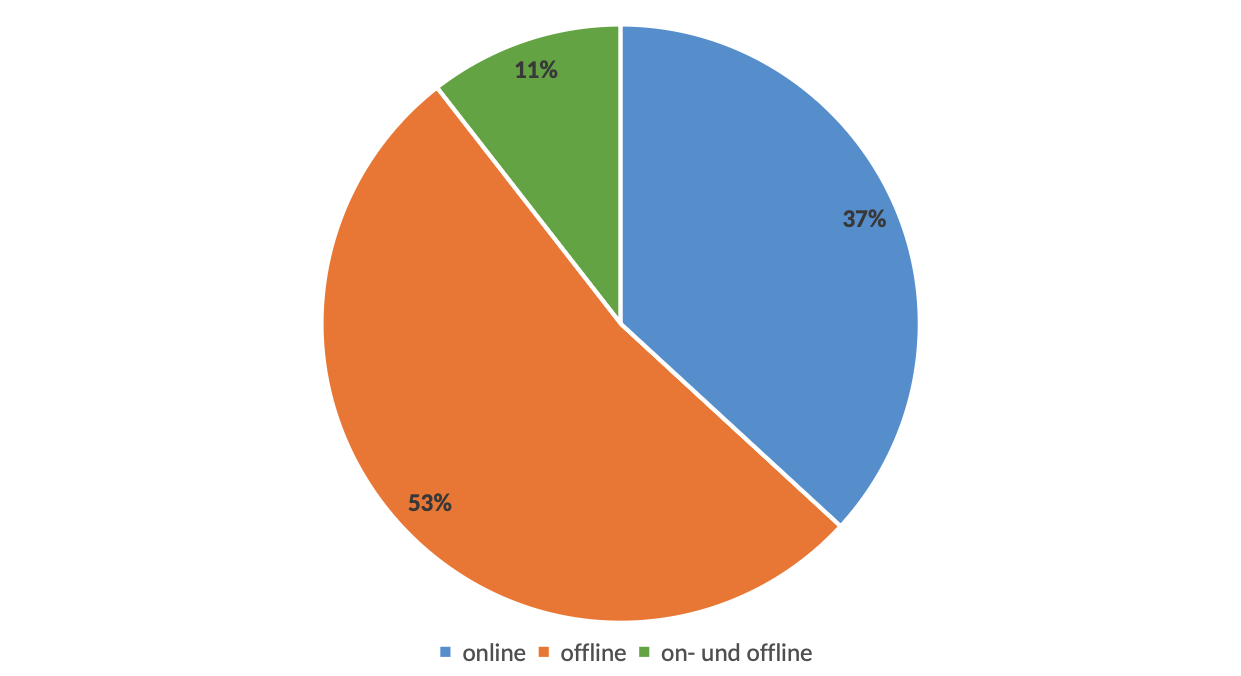
\includegraphics[width=0.90\textwidth]{graphics_sim/3-zugriff.png}
        \caption{Aufteilung Zugriff}
        \label{fig:3-zugriff-sim}
    \end{subfigure}
    \hfill
    % 
    % --- rechte Seite: Grafik ---
    \begin{subfigure}[b]{0.48\textwidth}
        \centering
        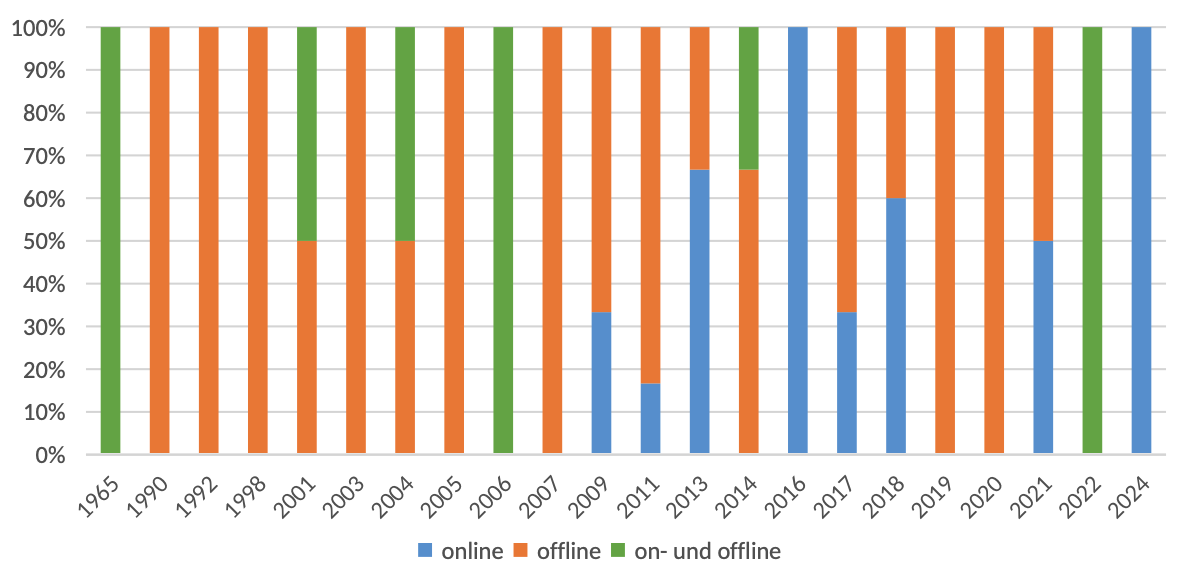
\includegraphics[width=0.90\textwidth]{graphics_sim/4-zugriff-jahr.png}
        \caption{Jährliche Aufteilung Zugriff}
        \label{fig:4-zugriff-jahr-sim}
    \end{subfigure}
    %
    \caption{Analysen zum Zugriff (Simulator)}
    \label{fig:zugriff-gesamt-sim}
\end{figure}

Bezogen auf das Kriterium \enquote{\acs{OS}} wird keine Abbildung dargestellt, da einzelne Simulatoren mehreren Betriebssystemen zugeordnet werden können. Stattdessen zeigt Tabelle~\ref{tab:os} die Verteilung der Systeme. Auffällig ist der hohe Anteil von Simulatoren in der Kategorie \enquote{unabhängig}, die online verfügbar und damit nicht an ein spezifisches Betriebssystem gebunden sind. Rund 65~\% dieser betriebssystemagnostischen Simulatoren wurden zwischen 2010 und 2020 veröffentlicht, während der Trend in den Folgejahren abflachte.

Tabelle~\ref{tab:os} zeigt darüber hinaus, dass etwa 37~\% der offline-nutzbaren Simulatoren die gängigen Betriebssysteme \enquote{Linux}, \enquote{Windows} und \enquote{macOS} unterstützen.

\begin{table}[h]
	\centering
	\caption{Verteilung der unterstützten Betriebssysteme (Simulator)}
	\label{tab:os}
	\begin{tabular}{l r}
		\toprule
		\textbf{Betriebssystem(e)} & \textbf{Anzahl} \\
		\midrule
		Linux                     & 4  \\
		Linux, Windows            & 1  \\
		Linux, Windows, macOS     & 11 \\
		Windows                   & 1  \\
		Windows, \ac{VM}          & 1  \\
		\ac{VM}                   & 2  \\
		unabhängig                & 37 \\
        \hline
        \textbf{Summe}            & \textbf{57} \\
		\bottomrule
	\end{tabular}
\end{table}

\sh{Preis}
Der überwiegende Teil der Simulatoren ist kostenfrei verfügbar; lediglich 5~\% sind kostenpflichtig. Eine Übersicht der Verteilung zeigt Abbildung~\ref{fig:9-preis}. Somit wird auch hier der finanzielle Druck auf Lehr- und Lernende reduziert.

\begin{figure}[!htbp]
    \centering
    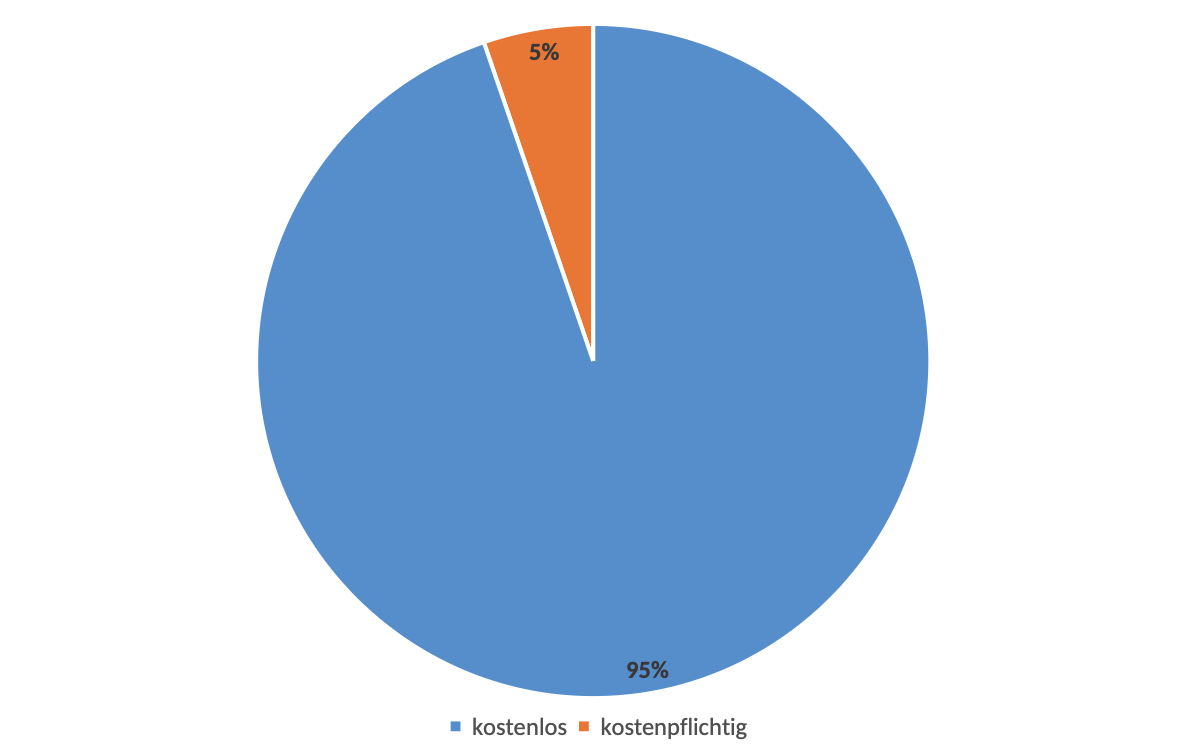
\includegraphics[width=0.90\textwidth]{graphics_sim/9-preis.png}
    \caption{Darstellung der Preisgestaltung (Simulator)}
    \label{fig:9-preis}
\end{figure}

\sh{Zeit}
Die Abbildungen~\ref{fig:12-zeit} und \ref{fig:13-vorwissen-thema} geben Aufschluss über die Nutzungsdauer der untersuchten Simulatoren. Der überwiegende Teil weist eine kurze Nutzungszeit auf, während lediglich 2~\% eine längere Bearbeitungsdauer vorsehen. In den Themenbereichen \enquote{Prozessoren und Architekturen} sowie \enquote{Hardware und Logik} finden sich ausschließlich Simulatoren mit kurzer Nutzungszeit.

\begin{figure}[!htbp]
    \centering
    % --- linke Seite: Grafik ---
    \begin{subfigure}[b]{0.48\textwidth}
        \centering
        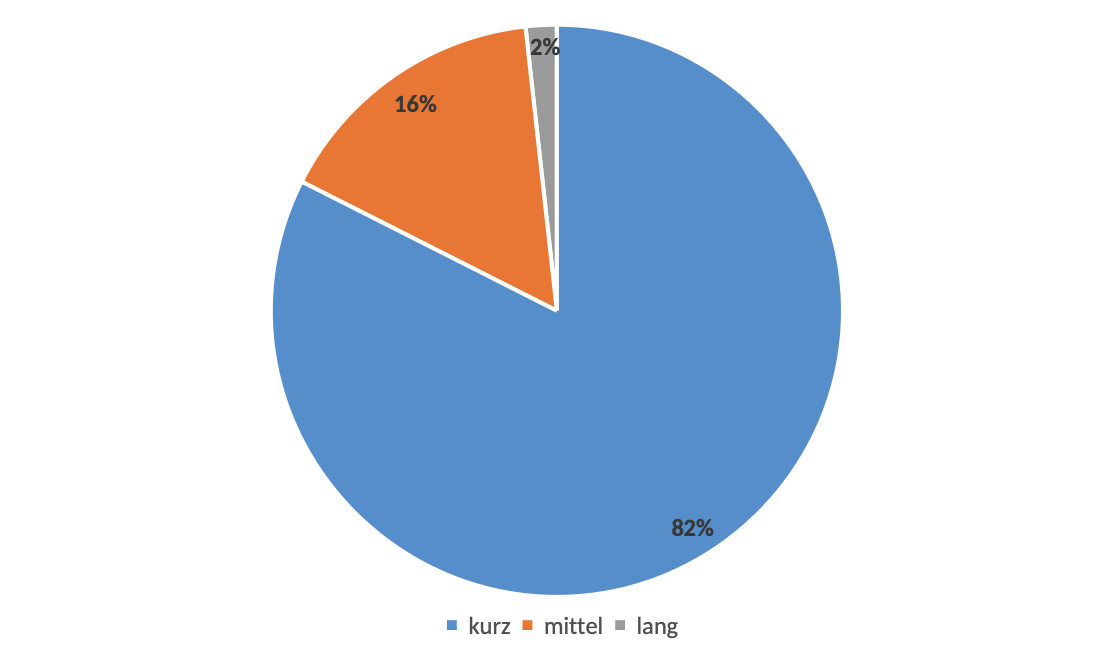
\includegraphics[width=0.90\textwidth]{graphics_sim/12-zeit.png}
        \caption{Verteilung Zeit}
        \label{fig:12-zeit}
    \end{subfigure}
    \hfill
    % 
    % --- rechte Seite: Grafik ---
    \begin{subfigure}[b]{0.48\textwidth}
        \centering
        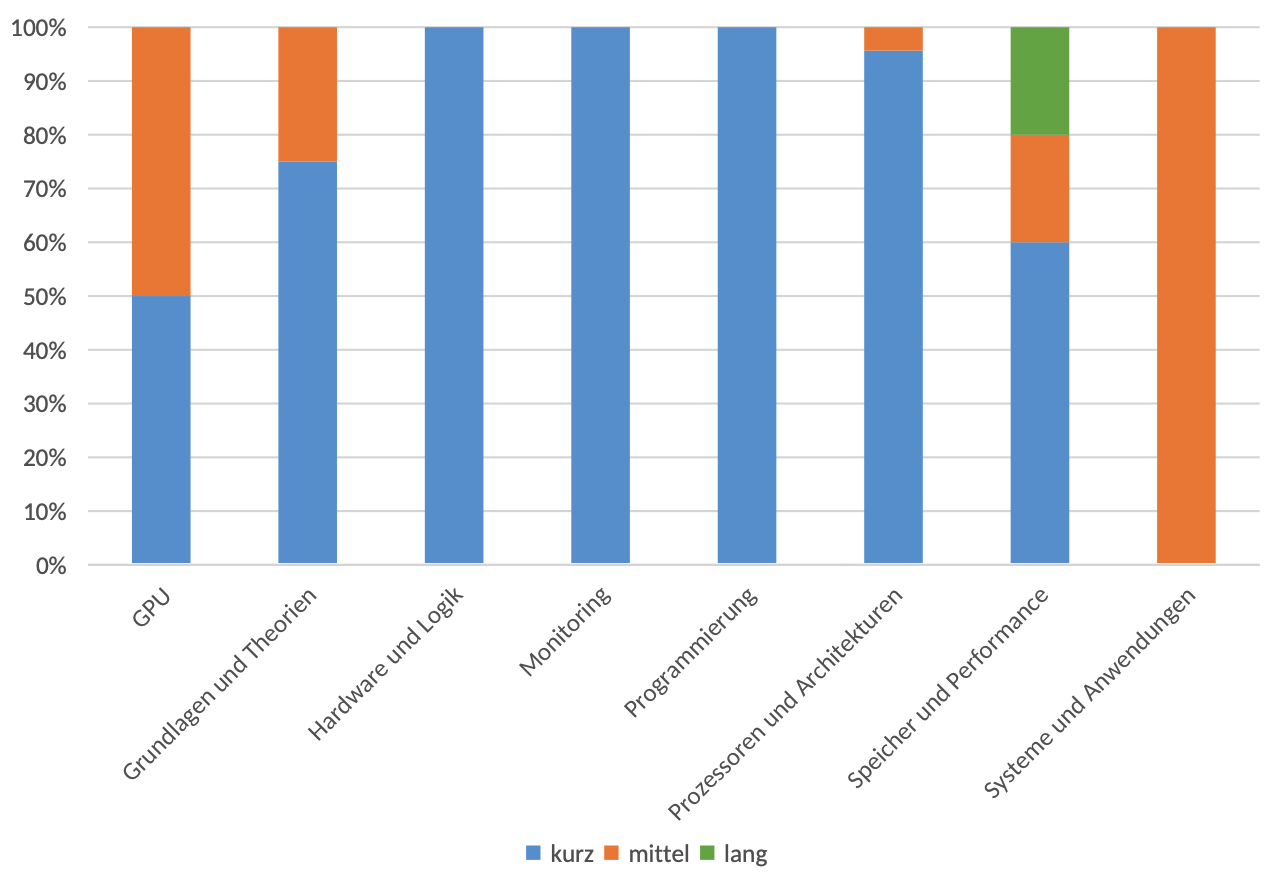
\includegraphics[width=0.90\textwidth]{graphics_sim/13-zeit-thema.png}
        \caption{Aufteilung Zeit nach Themen}
        \label{fig:13-vorwissen-thema}
    \end{subfigure}
    %
    \caption{Analysen zur Zeit (Simulator)}
    \label{fig:nutzungsdauer-gesamt}
\end{figure}

Die benötigte Bearbeitungszeit eines Simulators lässt sich mit den in Kapitel~\ref{chap:3-1-psychology} dargestellten lernpsychologischen Theorien in Beziehung setzen. Eine Analyse dieses Kriteriums ist daher zentral für die Ableitung zukünftiger Trends und Best Practices. 

Die Auswertung des erforderlichen Zeitaufwands (vgl. Abbildung~\ref{fig:12-zeit}) zeigt, dass die meisten Simulatoren bereits nach kurzer Nutzungsdauer zu Ergebnissen führen. Aus lernpsychologischer Perspektive ergeben sich daraus unterschiedliche Implikationen:


\begin{itemize}
    \item \textit{\ac{CTML}}: Kurze Bearbeitungszeiten können kognitive Überlastung verringern, bergen jedoch die Gefahr, dass für \textit{Active Processing} zu wenig Zeit verbleibt.
    \item \textit{Exploratives Lernen}: Eine geringe Nutzungsdauer schränkt die Möglichkeit ein, eigene Hypothesen ausführlich zu erproben.
    \item \textit{Erfahrungsbasiertes Lernen}: Für die Phase der \textit{reflektierenden Beobachtung} könnte die kurze Dauer unzureichend sein, um Erlebtes nachhaltig zu verarbeiten.
    \item \textit{Konnektivismus}: Die Integration neuer Informationen in bestehende Wissensnetzwerke erfordert mehr Zeit, als viele Simulatoren vorsehen.
\end{itemize}

Aus der Analyse der Nutzungsdauer in Bezug auf die Themen (vgl. Abbildung~\ref{fig:13-vorwissen-thema}) ergeben sich keine zusätzlichen Erkenntnisse. Die höhere Verteilung in den Kategorien \enquote{Hardware und Logik} sowie \enquote{Prozessoren und Architekturen} entspricht der bereits zuvor dargestellten allgemeinen Themenverteilung.

\sh{Dokumentation}
Die Analyse der Dokumentation zeigt (vgl. Abbildung~\ref{fig:14-dokumentation}), dass 88~\% der untersuchten Simulatoren über eine ausreichende Begleitdokumentation verfügen. Die lernpsychologischen Theorien verdeutlichen dabei die Bedeutung solcher Materialien, da sie den Lern- und Lehrprozess auf unterschiedlichen Ebenen unterstützen.

\begin{figure}[!htbp]
    \centering
    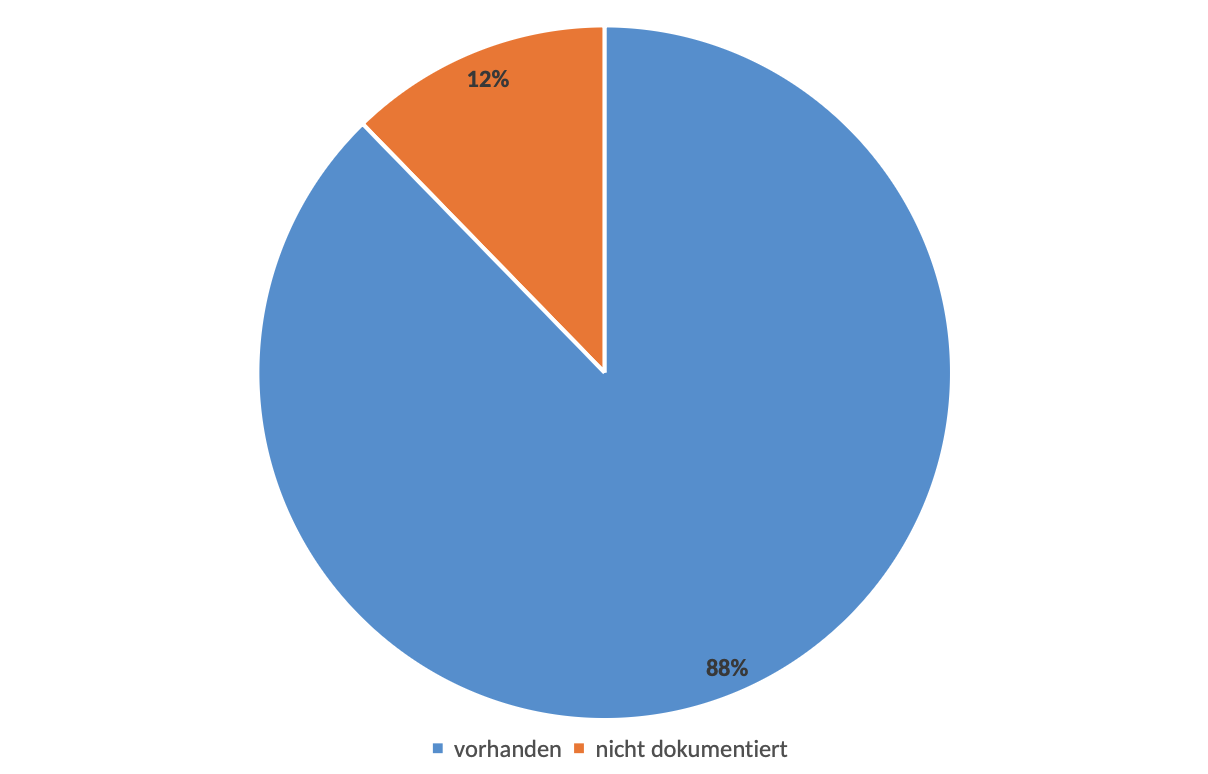
\includegraphics[width=0.90\textwidth]{graphics_sim/14-dokumentation.png}
    \caption{Verteilung der Dokumentation}
    \label{fig:14-dokumentation}
\end{figure}

\sh{Bekanntheit}
Als abschließendes Kriterium wird die Bekanntheit der Simulatoren betrachtet. Insgesamt werden 78~\% der Simulatoren als mittel oder hoch bekannt eingestuft (vgl. Abbildung~\ref{fig:15-bekanntheit}). Eine Übersicht darüber, welche Themenbereiche vergleichsweise geringere Bekanntheit aufweisen, bietet Abbildung~\ref{fig:16-bekanntheit-thema}.

\begin{figure}[!htbp]
    \centering
    % --- linke Seite: Grafik ---
    \begin{subfigure}[b]{0.48\textwidth}
        \centering
        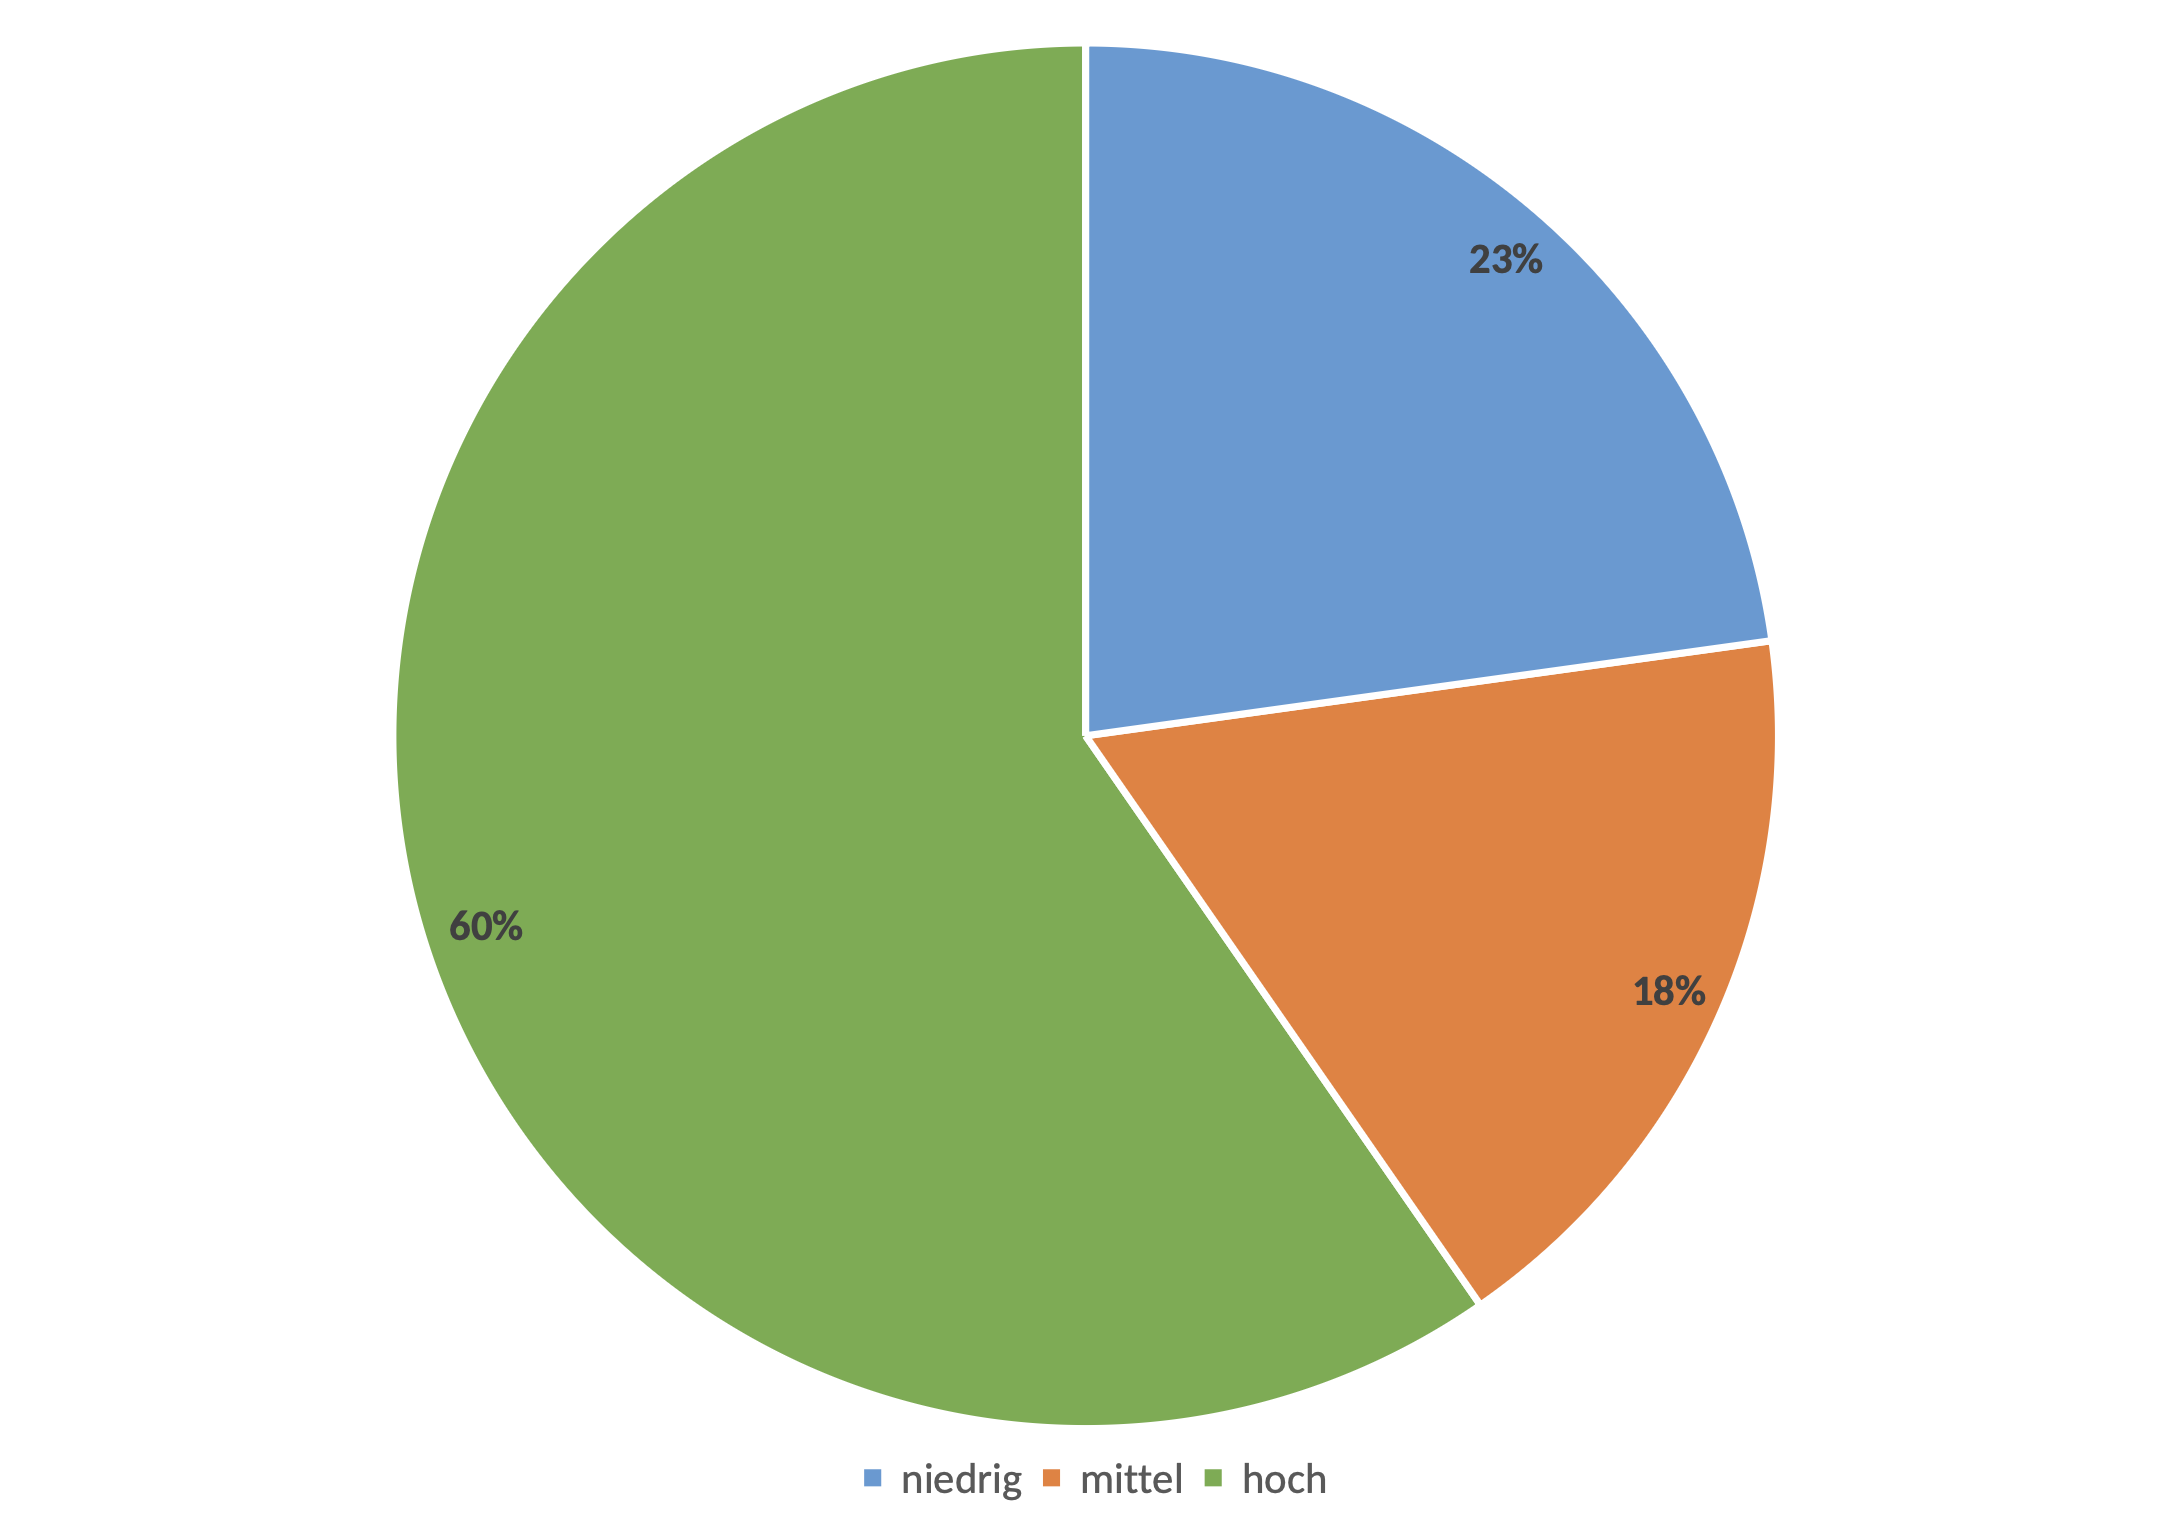
\includegraphics[width=0.90\textwidth]{paper/graphics_sim/15-bekanntheit2.png}
        \caption{Aufteilung Bekanntheit}
        \label{fig:15-bekanntheit}
    \end{subfigure}
    \hfill
    % 
    % --- rechte Seite: Grafik ---
    \begin{subfigure}[b]{0.48\textwidth}
        \centering
        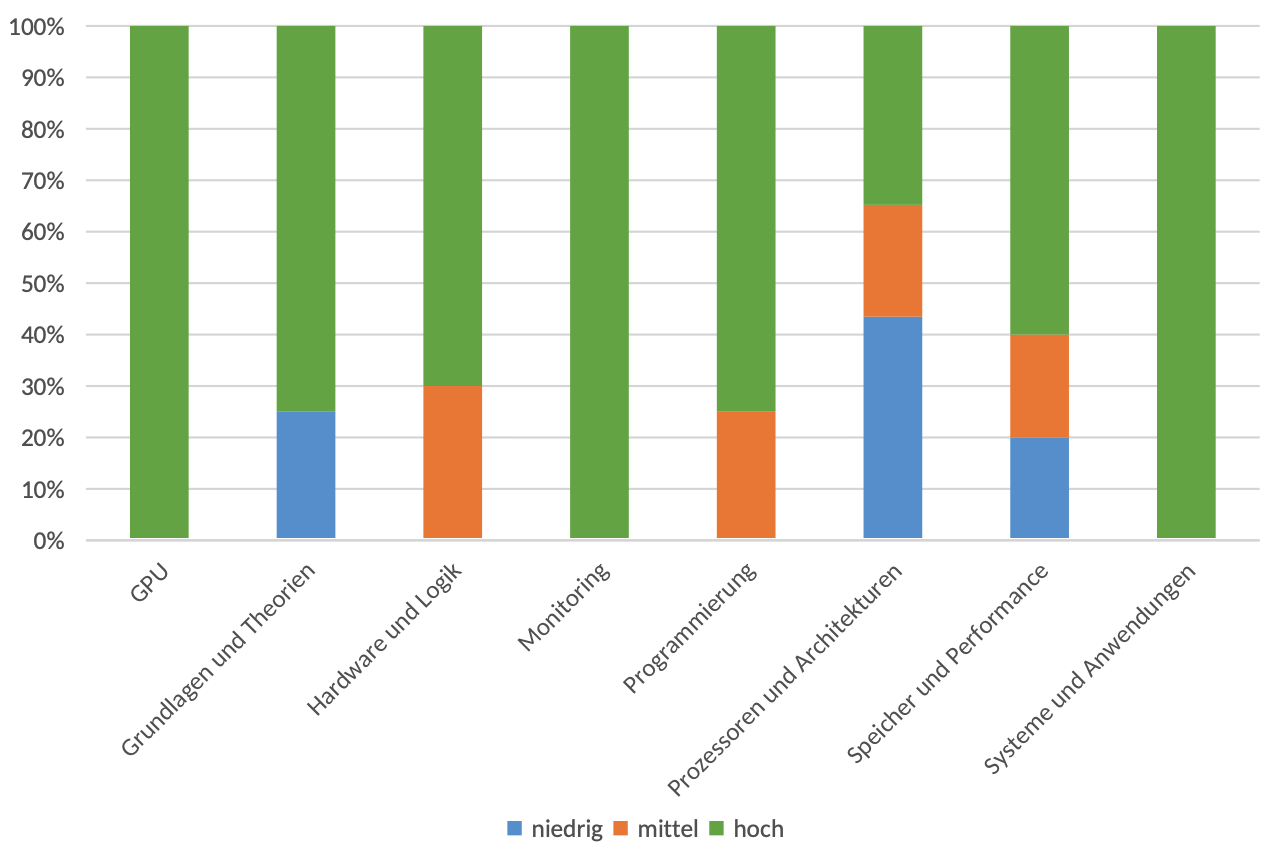
\includegraphics[width=0.90\textwidth]{graphics_sim/16-bekanntheit-thema.png}
        \caption{Aufteilung Bekanntheit auf Themen}
        \label{fig:16-bekanntheit-thema}
    \end{subfigure}
    %
    \caption{Analysen zur Bekanntheit (Simulator)}
    \label{fig:bekanntheit-gesamt}
\end{figure}

Abbildung~\ref{fig:16-bekanntheit-thema} zeigt, dass Simulatoren der Themenbereiche \enquote{GPU}, \enquote{Monitoring} sowie \enquote{Systeme und Anwendungen} zwar eine hohe Bekanntheit aufweisen, jedoch im didaktischen Hochschulkontext nur begrenzt eingesetzt werden. Eine mögliche Erklärung hierfür ist der stärker realitätsnahe Charakter dieser Simulatoren. Im Gegensatz dazu verfügen Simulatoren im Themenfeld \enquote{Speicher und Performance} insgesamt über eine geringere Bekanntheit.
